% id: 0272
% book: RPM 중3-2 수학 · 03 원과 직선
% section: 유형 02 현의 수직이등분선 (2)
% figure: crop:fig-0272.png
% answer: ③
% answer_source: 답지
% variant_level: 0 (원본 전사)
% 이 파일은 build.mjs 가 items.json 에서 만든다. 고칠 때는 items.json 을 고친다.
\noindent\begin{minipage}[t]{0.58\linewidth}\vspace{0pt}\raggedright 오른쪽 그림의 원~$\pt{O}$에서 $\seg{OD}\perp\seg{AB}$이고 $\seg{OC}=3\mkern3mu \mathrm{cm}$, $\seg{CD}=2\mkern3mu \mathrm{cm}$일 때, $\seg{AB}$의 길이는?\end{minipage}\hfill\begin{minipage}[t]{0.4\linewidth}\vspace{0pt}\centering \setlength{\dmfigw}{64.2pt}\ifdim\dmfigw>\linewidth\setlength{\dmfigw}{\linewidth}\fi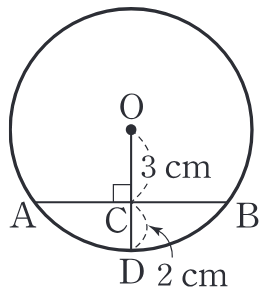
\includegraphics[width=\dmfigw]{figures/fig-0272.png}\end{minipage}\par
\begin{choicesii}{$6\mkern3mu \mathrm{cm}$}{$7\mkern3mu \mathrm{cm}$}{$8\mkern3mu \mathrm{cm}$}{$9\mkern3mu \mathrm{cm}$}{$10\mkern3mu \mathrm{cm}$}\end{choicesii}
